\documentclass[9pt,twocolumn,twoside,]{pnas-new}

% Use the lineno option to display guide line numbers if required.
% Note that the use of elements such as single-column equations
% may affect the guide line number alignment.


\usepackage[T1]{fontenc}
\usepackage[utf8]{inputenc}

% tightlist command for lists without linebreak
\providecommand{\tightlist}{%
  \setlength{\itemsep}{0pt}\setlength{\parskip}{0pt}}


% Pandoc citation processing
\newlength{\cslhangindent}
\setlength{\cslhangindent}{1.5em}
\newlength{\csllabelwidth}
\setlength{\csllabelwidth}{3em}
\newlength{\cslentryspacingunit} % times entry-spacing
\setlength{\cslentryspacingunit}{\parskip}
% for Pandoc 2.8 to 2.10.1
\newenvironment{cslreferences}%
  {}%
  {\par}
% For Pandoc 2.11+
\newenvironment{CSLReferences}[2] % #1 hanging-ident, #2 entry spacing
 {% don't indent paragraphs
  \setlength{\parindent}{0pt}
  % turn on hanging indent if param 1 is 1
  \ifodd #1
  \let\oldpar\par
  \def\par{\hangindent=\cslhangindent\oldpar}
  \fi
  % set entry spacing
  \setlength{\parskip}{#2\cslentryspacingunit}
 }%
 {}
\usepackage{calc}
\newcommand{\CSLBlock}[1]{#1\hfill\break}
\newcommand{\CSLLeftMargin}[1]{\parbox[t]{\csllabelwidth}{#1}}
\newcommand{\CSLRightInline}[1]{\parbox[t]{\linewidth - \csllabelwidth}{#1}\break}
\newcommand{\CSLIndent}[1]{\hspace{\cslhangindent}#1}


\templatetype{pnasresearcharticle}  % Choose template

\title{Rapport sur les interactions entre étudiants de l'Université de
Sherbrooke}

\author[a,1,2]{Gabrielle Beauchesne}
\author[a,b]{Magalie Bossé}
\author[a,b,c]{Amélie Pelletier}

  \affil[]{}


% Please give the surname of the lead author for the running footer
\leadauthor{}

% Please add here a significance statement to explain the relevance of your work
\significancestatement{}


\authorcontributions{}



\correspondingauthor{\textsuperscript{} }

% Keywords are not mandatory, but authors are strongly encouraged to provide them. If provided, please include two to five keywords, separated by the pipe symbol, e.g:
 \keywords{  interactions |  écologie |  communautés  } 

\begin{abstract}
Please provide an abstract of no more than 250 words in a single
paragraph. Abstracts should explain to the general reader the major
contributions of the article. References in the abstract must be cited
in full within the abstract itself and cited in the text.
\end{abstract}

\dates{This manuscript was compiled on \today}
\doi{\url{www.pnas.org/cgi/doi/10.1073/pnas.XXXXXXXXXX}}

\begin{document}

% Optional adjustment to line up main text (after abstract) of first page with line numbers, when using both lineno and twocolumn options.
% You should only change this length when you've finalised the article contents.
\verticaladjustment{-2pt}



\maketitle
\thispagestyle{firststyle}
\ifthenelse{\boolean{shortarticle}}{\ifthenelse{\boolean{singlecolumn}}{\abscontentformatted}{\abscontent}}{}

% If your first paragraph (i.e. with the \dropcap) contains a list environment (quote, quotation, theorem, definition, enumerate, itemize...), the line after the list may have some extra indentation. If this is the case, add \parshape=0 to the end of the list environment.

\acknow{}

\hypertarget{introduction}{%
\subsection*{Introduction}\label{introduction}}
\addcontentsline{toc}{subsection}{Introduction}

Dans le baccalauréat en biologie à l'Université de Sherbrooke, il est
possible de s'inscrire à un des quatre programmes présentés soit :
biologie générale, biologie cellulaire, écologie et microbiologie. À
travers ces différents programmes, il y a chevauchement de plusieurs
cours entrainant ainsi des interactions multiples entre les étudiants de
ces quatre programmes. Les interactions sont également possibles dans
des cours optionnels où d'autres programmes viennent s'ajouter à ces
quatre programmes. D'où la question : est-ce que les propriétés du
réseau de collaboration entre étudiants en écologie diffèrent de celles
d'un réseau écologique ? Il sera donc question d'évaluation des
interactions produites par chaque membre pour représenter le réseau de
collaboration des étudiants puis de comparer ce réseau avec des réseaux
écologiques.

\hypertarget{Muxe9thodologie}{%
\subsection*{Méthodologie}\label{Muxe9thodologie}}
\addcontentsline{toc}{subsection}{Méthodologie}

Concernant la méthodologie, la classe a été divisée en plusieurs équipes
de 3 à 4 personnes pour monter leur propre fichier de données concernant
les collaborations effectuées par chaque membre de l'équipe depuis le
début de leur baccalauréat. Certaines données supplémentaires concernant
les cours auxquels chacun a participé ainsi que les renseignements sur
chaque membre de l'équipe, programme choisi, session de début, etc. ont
été compilés en même temps que les collaborations. Par la suite, nous
avons combiner les données de chaque équipe pour former trois grandes
tables : cours, étudiant et collaboration. Nous avons nettoyé les tables
puis opérer diverses manœuvres dans R pour effectuer nos analyses. Nous
avons créé des requêtes SQL pour nos analyses et pour visualiser
celles-ci. Un fichier target a également été conçu. Finalement, nous
avons utiliser RMarkdown pour la mise en page de ce rapport.

\hypertarget{Ruxe9sultats}{%
\subsection*{Résultats}\label{Ruxe9sultats}}
\addcontentsline{toc}{subsection}{Résultats}

Comme on peut voir à la figure 1, les sessions avec le plus de
collaborations étaient en hiver 2021 et en hiver 2023. Les sessions avec
le moins de collaborations étaient en été 2021 et à l'automne 2020.\\
À la figure 2, on constate que les cours TSB 303 et BCM 104 faisaient
parti des cours avec le plus de collaborations tandis que ALM 300 et BCM
111 étaient certains des cours avec le moins de collaborations entre les
étudiants.

\hypertarget{references}{%
\subsection*{Tableaux}\label{references}}
\addcontentsline{toc}{subsection}{Tableaux}

\begin{figure*}
  \centering
  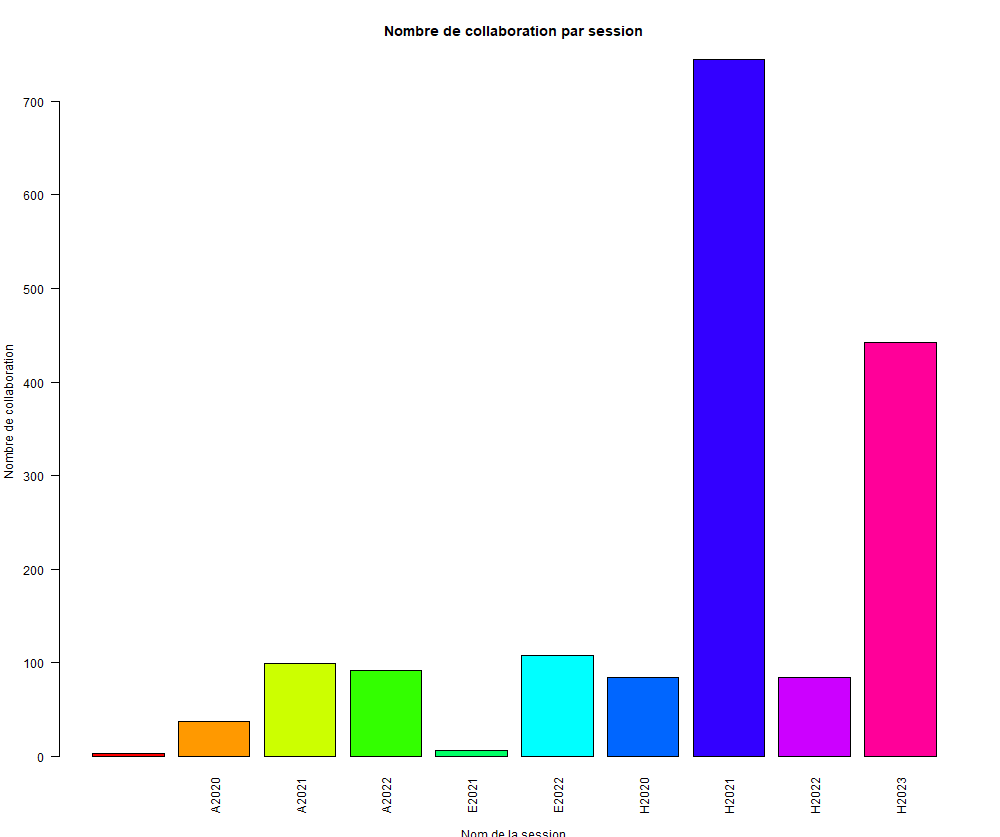
\includegraphics[width=\linewidth]{session.png}
  \caption{Légende de l'image}
  \label{fig:session}
\end{figure*}

\begin{figure*}
  \centering
  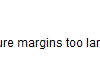
\includegraphics[width=\linewidth]{sigle.png}
  \caption{Légende de l'image}
  \label{fig:sigle}
\end{figure*}

\hypertarget{Discussion}{%
\subsection*{Discussion}\label{Discussion}}
\addcontentsline{toc}{subsection}{Discussion}

Dans une communauté écologique plusieurs interactions peuvent subvenir
entre les individus. C'est le même principe pour les étudiants de
l'université. Dans l'écologie des communautés, on parle de richesse
spécifique pour décrire le nombre d'espèces présentes sur le lieu de
l'étude. Pour les étudiants, la richesse spécifique serait en fait le
nombre d'étudiants présent dans le cours de méthode en écologie
computationnelle. Il est possible en utilisant les liens effectués entre
les différentes espèces ou entre les étudiants de produire une matrice
d'adjacence qui décrirait les interactions entre les individus ainsi que
le niveau d'interaction entre ces individus (1). Pour différencier les
types d'interactions on peut utiliser des réseaux binaires qui ne
décrivent pas la direction du lien en question. On peut aussi utiliser
des réseaux directionnels et valués qui permettent de décrire la
direction de l'interaction et son intensité séparément. Ces réseaux sont
utiles pour décrire des interactions fortes ou des interactions
différentes en fonction du sens de l'interaction. Dans une communauté
écologique, une relation de prédation de l'espèce 1 à l'espèce 2 ne sera
pas représenté de la même façon dans un réseau directionnel par exemple
(2). Dans l'étude réalisée ici, on se contentera d'utiliser des
interactions binaires entre les étudiants étant donné qu'on ne
différencie pas le type d'interaction. En écologie des communautés on
parle de degré de nœud pour décrire le nombre de liens qu'une espèce
fait avec d'autres espèces. Plus il y a de liens d'effectuées, plus le
degré du nœud sera élevé. Il est possible de retrouver la même logique
dans les relations entre étudiants. Certains étudiants ont tendances à
former plus de liens avec leurs pairs que d'autres. Les étudiants qui
ont plusieurs interactions avec plusieurs élèves différents seront les
nœuds centraux de la matrice. En effet, ce sont eux qui permettent de
former le plus d'interactions entre les étudiants (2). Plus un nœud est
central et avec un degré élevé, plus son retrait dans une communauté
écologique impactera le réseau. Le même principe peut être appliqué aux
étudiants de l'université. Si on retire les étudiants centraux de notre
réseau, plusieurs interactions entres d'autres étudiants ne seraient
possiblement pas survenues (3). Plusieurs types d'interactions peuvent
survenir dans un milieu écologique. On retrouve par exemple de la
prédation, des interactions symbiotiques, du commensalisme et plusieurs
autres (3). Chez les étudiants de l'université, on observe surtout des
interactions qui se rapprochent d'une symbiose en écologie. En effet,
certains étudiants ont plutôt tendance à former des groupes pour
s'entraider et on observe de grandes quantités d'interactions à
l'intérieur de ces groupes en question.

\hypertarget{Conclusion}{%
\subsection*{Conclusion}\label{Conclusion}}
\addcontentsline{toc}{subsection}{Conclusion}

Il est possible de dire que les interactions entres les étudiants de
l'université est comparable dans certaines mesures à un système
d'interaction d'une communauté écologique. En effet, dans les deux cas
on observe une tendance à former des groupes symbiotiques dans lesquels
on observe une grande quantité d'interactions entre les entités. Aussi,
dans les deux cas on observe un fort impact du retrait des nœuds
centraux sur les interactions dans la communauté. Pour pousser
d'avantage la réflexion, il serait possible de tenter d'inclure dans
l'analyse le type d'interaction entre les étudiants. Par exemple, ces
interactions pourraient être de l'entraide, de l'aide donnée par un
étudiant à un autre ou encore des mésentendus entres étudiants. Ainsi,
il pourrait être possible de pousser les analyses pour déterminer non
seulement si les réseaux d'interactions sont comparables, mais aussi si
les types d'interactions sont régis de la même façon entre les deux
types de communautés.

\hypertarget{appendices}{%
\subsubsection*{Appendices}\label{appendices}}
\addcontentsline{toc}{subsubsection}{Appendices}

\showmatmethods
\showacknow
\pnasbreak

\hypertarget{refs}{}
\begin{CSLReferences}{0}{0}
\leavevmode\vadjust pre{\hypertarget{ref-saavedra_structural_2017}{}}%
\CSLLeftMargin{1. }%
\CSLRightInline{Saavedra S, et al. (2017)
\href{https://doi.org/10.1002/ecm.1263}{A structural approach for
understanding multispecies coexistence}. \emph{Ecological Monographs}
87(3):470--486.}

\leavevmode\vadjust pre{\hypertarget{ref-delmas_analysing_2019}{}}%
\CSLLeftMargin{2. }%
\CSLRightInline{Delmas E, et al. (2019)
\href{https://doi.org/10.1111/brv.12433}{Analysing ecological networks
of species interactions: {Analyzing} ecological networks}.
\emph{Biological Reviews} 94(1):16--36.}

\leavevmode\vadjust pre{\hypertarget{ref-berquer_analyse_nodate}{}}%
\CSLLeftMargin{3. }%
\CSLRightInline{Berquer A Analyse des réseaux d'interactions
plantes-pollinisateurs: {Concepts} et {Méthodes}.}

\end{CSLReferences}



% Bibliography
% \bibliography{pnas-sample}

\end{document}
